%%%%%%%%%%%%%%
%% Run LaTeX on this file several times to get Table of Contents,
%% cross-references, and citations.

%% w-bktmpl.tex. Current Version: Feb 16, 2012
%%%%%%%%%%%%%%%%%%%%%%%%%%%%%%%%%%%%%%%%%%%%%%%%%%%%%%%%%%%%%%%%
%
%  Template file for
%  Wiley Book Style, Design No.: SD 001B, 7x10
%  Wiley Book Style, Design No.: SD 004B, 6x9
%
%  Prepared by Amy Hendrickson, TeXnology Inc.
%  http://www.texnology.com
%%%%%%%%%%%%%%%%%%%%%%%%%%%%%%%%%%%%%%%%%%%%%%%%%%%%%%%%%%%%%%%%

%%%%%%%%%%%%%%%%%%%%%%%%%%%%%%%%%%%%%%%%%%%%%%%%%%%%%%%%%%%%%%%%
%% Class File

%% For default 7 x 10 trim size:
%\documentclass{WileySev}

%% Or, for 6 x 9 trim size
\documentclass{WileySix}
\usepackage[bookmarks,bookmarksopen,bookmarksdepth=2,colorlinks, citecolor=black, linkcolor=black, urlcolor=black]{hyperref}

\usepackage[figure]{hypcap}

%%%%%%%%%%%%%%%%%%%%%%%%%%%%%%%%%%%%%%%%%%%%%%%%%%%%%%%%%%%%%%%%
%% Post Script Font File

% For PostScript text
% If you have font problems, you may edit the w-bookps.sty file
% to customize the font names to match those on your system.

\usepackage{w-bookps}
\usepackage{amsmath}
%%%%%%%
%% For times math: However, this package disables bold math (!)
%% \mathbf{x} will still work, but you will not have bold math
%% in section heads or chapter titles. If you don't use math
%% in those environments, mathptmx might be a good choice.

% \usepackage{mathptmx}


%%%%%%%%%%%%%%%%%%%%%%%%%%%%%%%%%%%%%%%%%%%%%%%%%%%%%%%%%%%%%%%%
%% Graphicx.sty for Including PostScript .eps files

\usepackage{graphicx}

%%%%%%%%%%%%%%%%%%%%%%%%%%%%%%%%%%%%%%%%%%%%%%%%%%%%%%%%%%%%%%%%
%% Other packages you might want to use:

% for chapter bibliography made with BibTeX
% \usepackage{chapterbib}

% for multiple indices
% \usepackage{multind}

% for answers to problems
% \usepackage{answers}

%%%%%%%%%%%%%%%%%%%%%%%%%%%%%%%%%%%%%%%%%%%%%%%%%%%%%%%%%%%%%%%%
%% Change options here if you want:
%%
%% How many levels of section head would you like numbered?
%% 0= no section numbers, 1= section, 2= subsection, 3= subsubsection
%%==>>
\setcounter{secnumdepth}{3}

%% How many levels of section head would you like to appear in the
%% Table of Contents?
%% 0= chapter titles, 1= section titles, 2= subsection titles, 
%% 3= subsubsection titles.
%%==>>
\setcounter{tocdepth}{2}

%% Cropmarks? good for final page makeup
%% \docropmarks %% turn cropmarks on

%%%%%%%%%%%%%%%%%%%%%%%%%%%%%%%%%%%%%%%%%%%%%%%%%%%%%%%%%%%%%%%%
%% DRAFT
%
% Uncomment to get double spacing between lines, current date and time
% printed at bottom of page.
% \draft
% (If you want to keep tables from becoming double spaced also uncomment
% this):
% \renewcommand{\arraystretch}{0.6}
%%%%%%%%%%%%%%%%%%%%%%%%%%%%%%
\newcommand{\apricot}{\bfseries Apricot}
\begin{document}

%%%%%%%%%%%%%%%%%%%%%%%%%%%%%%%%%%%%%%%%%%%%%%%%%%%%%%%%%%%%%%%%
%% Title Pages
%%
%% Wiley will provide title and copyright page, but you can make
%% your own titlepages if you'd like anyway

%% Setting up title pages, type in the appropriate names here:
\booktitle{Apricot User Guider}
%\subtitle{An Approach for Hybrid Systems}

\author{~~FANG HUI-XING\\
%\affil{APRICOTRESEARCH.COM}
}
%or
%\authors{FANG HUIXING}

%% \\ will start a new line.
%% You may add \affil{} for affiliation, ie,
%\authors{Robert M. Groves\\
%\affil{Universitat de les Illes Balears}
%Floyd J. Fowler, Jr.\\
%\affil{University of New Mexico}
%}

%% Print Half Title and Title Page:
\halftitlepage
\titlepage


%%%%%%%%%%%%%%%%%%%%%%%%%%%%%%%%%%%%%%%%%%%%%%%%%%%%%%%%%%%%%%%%
%% Off Print Info

%% Add your info here:
\offprintinfo{Apricot User Guider, apricotresearch.com}{FANG Hui-Xing}

%% Can use \\ if title, and edition are too wide, ie,
%% \offprintinfo{Survey Methodology,\\ Second Edition}{Robert M. Groves}


%%%%%%%%%%%%%%%%%%%%%%%%%%%%%%%%%%%%%%%%%%%%%%%%%%%%%%%%%%%%%%%%
%% Copyright Page

\begin{copyrightpage}{2013}
Apricot User Guider, etc
\end{copyrightpage}

% Note, you must use \ to start indented lines, ie,
% 
% \begin{copyrightpage}{2004}
% Survey Methodology / Robert M. Groves . . . [et al.].
% \       p. cm.---(Wiley series in survey methodology)
% \    ``Wiley-Interscience."
% \    Includes bibliographical references and index.
% \    ISBN 0-471-48348-6 (pbk.)
% \    1. Surveys---Methodology.  2. Social 
% \  sciences---Research---Statistical methods.  I. Groves, Robert M.  II. %
% Series.\\

% HA31.2.S873 2004
% 001.4'33---dc22                                             2004044064
% \end{copyrightpage}

%%%%%%%%%%%%%%%%%%%%%%%%%%%%%%%%%%%%%%%%%%%%%%%%%%%%%%%%%%%%%%%%
%% Frontmatter >>>>>>>>>>>>>>>>

%%%%%%%%%%%%%%%%%%%%%%%%%%%%%%%%%%%%%%%%%%%%%%%%%%%%%%%%%%%%%%%%
%% Only Dedication (optional) 
%% or Contributor Page for edited books
%% before \tableofcontents

\dedication{To my parents and friends}

% ie,
%\dedication{To my parents}

%%%%%%%%%%%%%%%%%%%%%%%%%%%%%%%%%%%%%%%%%%%%%%%%%%%%%%%%%%%%%%%%
%  Contributors Page for Edited Book
%%%%%%%%%%%%%%%%%%%%%%%%%%%%%%%%%%%%%%%%%%%%%%%%%%%%%%%%%%%%%%%%

% If your book has chapters written by different authors,
% you'll need a Contributors page.

% Use \begin{contributors}...\end{contributors} and
% then enter each author with the \name{} command, followed
% by the affiliation information.

% \begin{contributors}
% \name{Masayki Abe,} Fujitsu Laboratories Ltd., Fujitsu Limited, Atsugi,
% Japan

% \name{L. A. Akers,} Center for Solid State Electronics Research, Arizona
% State University, Tempe, Arizona

% \name{G. H. Bernstein,} Department of Electrical and
% Computer Engineering, University of Notre Dame, Notre Dame, South Bend, 
% Indiana; formerly of
% Center for Solid State Electronics Research, Arizona
% State University, Tempe, Arizona 
% \end{contributors}

%%%%%%%%%%%%%%%%%%%%%%%%%%%%%%%%%%%%%%%%%%%%%%%%%%%%%%%%%%%%%%%%
\contentsinbrief %optional

\tableofcontents 

 \listoffigures %optional
 \listoftables  %optional

%%%%%%%%%%%%%%%%%%%%%%%%%%%%%%%%%%%%%%%%%%%%%%%%%%%%%%%%%%%%%%%%
% Optional Foreword:

\begin{foreword}
%text
\end{foreword}

%%%%%%%%%%%%%%%%%%%%%%%%%%%%%%%%%%%%%%%%%%%%%%%%%%%%%%%%%%%%%%%%
% Optional Preface:

%\begin{preface}
% text
%\prefaceauthor{}
%\where{place\\
% date}
%\end{preface}

% ie,
% \begin{preface}
% This is an example preface.
% \prefaceauthor{R. K. Watts}
% \where{Durham, North Carolina\\
% September, 2004}

%%%%%%%%%%%%%%%%%%%%%%%%%%%%%%%%%%%%%%%%%%%%%%%%%%%%%%%%%%%%%%%%
% Optional Acknowledgments:

% \acknowledgments
% acknowledgment text
% \authorinitials{} % ie, I. R. S.


%%%%%%%%%%%%%%%%%%%%%%%%%%%%%%%%
%% Glossary Type of Environment:

% \begin{glossary}
% \term{<term>}{<description>}
% \end{glossary}

%%%%%%%%%%%%%%%%%%%%%%%%%%%%%%%%
% \begin{acronyms} 
% \acro{<term>}{<description>}
% \end{acronyms}

%%%%%%%%%%%%%%%%%%%%%%%%%%%%%%%%
%% In symbols environment <term> is expected to be in math mode; 
%% if not in math mode, use \term{\hbox{<term>}}

% \begin{symbols}
% \term{<math term>}{<description>}
% \term{\hbox{<non math term>}}Box used when not using a math symbol.
% \end{symbols}

%%%%%%%%%%%%%%%%%%%%%%%%%%%%%%%%
 \begin{introduction}
%\introauthor{<name>}{<affil>}
% Introduction text...
 \end{introduction}

%%%%%%%%%%%%%%%%%%%%%%%%%%%%%%%%%%%%%%%%%%%%%%%%%%%%%%%%%%%%%%%%
%% End for Front Matter, Beginning of text of book  >>>>>>>>>>>

%% Short version of title without \\ may be written in sq. brackets:

%% Optional Part :
\part[The Modeling Language]{The Modeling Language}

\chapter[The Syntax of Apricot]{The Syntax of Apricot}

\section{Identifiers} 
An identifier is an unlimited-length (but the length is greater than one) sequence of letters and digits, but not a Keyword:


\begin{eqnarray*}
 Letter  &::=& {\tt a .. z \mid A .. Z} ;\\
 Digit  &::=& {\tt 0 .. 9};\\
 ValidChar  &::=&  Letter   ~\mid~  Digit ;\\
 Identifier  &::=& {\tt \verb!^!} ? (~Letter~|~{\tt \_}~) (~ValidChar~|~{\tt \_}~)*;.
\end{eqnarray*}


In which the letter is defied as the character in the set 
$\{$  ${\tt a}$, 
${\tt b}$, ${\tt c}$, ${\tt d}$, 
${\tt e}$, ${\tt f}$, ${\tt g}$, ${\tt h}$, 
${\tt i}$, ${\tt j}$, ${\tt k}$, ${\tt l}$, ${\tt m}$, 
${\tt n}$, ${\tt o}$, ${\tt p}$, ${\tt q}$, ${\tt r}$, 
${\tt s}$, ${\tt t}$, ${\tt u}$, ${\tt v}$, ${\tt w}$, 
${\tt x}$, ${\tt y}$, ${\tt z}$, ${\tt A}$, ${\tt B}$, 
${\tt C}$, ${\tt D}$, ${\tt E}$, ${\tt F}$, ${\tt G}$, 
${\tt H}$, ${\tt I}$, ${\tt J}$, ${\tt K}$, ${\tt L}$, 
${\tt M}$, ${\tt N}$, ${\tt O}$, ${\tt P}$, ${\tt Q}$, 
${\tt R}$, ${\tt S}$, ${\tt T}$, ${\tt U}$, ${\tt V}$, 
${\tt W}$, ${\tt X}$, ${\tt Y}$, ${\tt Z}$
$\}$.


\section{Types, Values, and Variables}
The types of the Apricot  language are divided into three categories: primitive types,
mathematic types and reference types. 

\begin{align*}
 Type ::= & PrimitiveType \mid MathematicType  \mid  ReferenceType ;\\
\end{align*}

\subsection{Primitive Types}


The primitive type is defined by:
\begin{eqnarray*}
 PrimitiveType &::=&  {\tt int} \mid {\tt real} \mid {\tt boolean} \mid {\tt String};\\
\end{eqnarray*}
The Boolean
type represents a logical quantity in the literals set $\{ {\tt true}, {\tt false}\}$.

\subsection{Mathematic Types and Values}
Primitive type variable 
can not be shared and has the feature of ``call-by-value" during method calls. 
Call-by-value requires the evaluation of the arguments before passing them to the definition of the method. Another style is call-by-name which passing the arguments directly to the definition.
For mathematic and reference types we take the call-by-name style argument passing for method invocation. In addition, there is a difference between mathematic type and reference type. Reference type variables can refer to another object with the same type by the assignment statement. But, the assignment can only change the mathematical value of the object for mathematic type variables. It means that, when a mathematic type variable refers to a methematic type object for the first time, the variable will hold this object all the time and only the mathematical value of this object can be updated.

\begin{eqnarray*}
 MathematicType  &::=&   {\tt Int} \mid {\tt Real};\\
\end{eqnarray*}

\begin{enumerate}
\item Mathematic types : Numeric types. 
The numeric types are the integer type Int, and the real number type
Real;
\item  Reference types : class types, interface types, and array types.
\end{enumerate}




An object is a dynamically created instance of a class type or a dynamically 
created array. The values of a reference type are references to objects.

\subsection{Reference Types and Values}

There are four kinds of reference types: class types, interface types, type variables.

\begin{align*}
 ReferenceType  ::=&  ClassType  \mid  InterfaceType   \\
                   &  \mid  ArrayType \mid IntervalType ;\\
 ClassType  ::=&  Identifier ;\\
 InterfaceType  ::=&  Identifier  \mid {\tt System} \mid {\tt Plant} \\
& \mid  {\tt Controller}\\
& \mid {\tt Dynamic} \mid {\tt Assignment} \\
& \mid {\tt ParallelAssignment} \\
& \mid {\tt SequentialAssignment} 
\end{align*}


\subsection{Variables}

A variable is a physical quantity name in physical world or a storage location in the memory of computer, and has an associated type that is either a mathematic type or a reference type.

The value of a variable  is changed by an assignment or according to the differential equations defined in {\em Dynamic} classes.

For all types, the default value of any type variable is the special value ${\tt null}$.

\subsubsection{Variables of Mathematic Type}
Mathematic type variables are always hold a mathematic value of that exact mathematic type.


\subsubsection{Variables of Reference Type}
A variable of a reference type ${\tt R}$ can hold a null reference, a reference to an instance of class {\em C}, any class that is a subclass of {\em C}, any class that is a implementation of interface {\em C} or any array type.



\section{Mathematical Operations}

\subsection{Arithmetic Operators}
For $x,y \in \mathcal{R}$, the following arithmetic operators are defined on Real numbers ($\mathcal{R}$):

\begin{enumerate}
\item  $x + y$,  binary plus, addition;
\item  $x - y$,  binary minus,subtraction;
\item  $x * y$,  binary multiple, multiplication;
\item  $x / y$,  binary divide, division;
\item  $+x$, unary plus, it denotes the identity operation on $x$, thus, $x == +x$ with
 respect to the evaluation;
\item  $-x$,  unary minus, inverse operation on $x$, thus, $(-x) + x == 0$.
\end{enumerate}





\subsection{Boolean Operators}
Standard boolean operators are defined for all *Boolean* type values $x, y$:

\begin{enumerate}
\item $==$, equality;

\item $!=$,  inequality;

\item $!$, logical complement;

\item ${\tt in}$,  belong to interval, the result value of ($x~ {\tt in}~[a,b]$) is ${\tt true}$ iff $a \leq x \leq b$;

\item ${\tt and}$, the result value of ($x~{\tt and}~y$) is ${\tt true}$ if both operand values are ${\tt true}$;

\item ${\tt xor}$, the result value of ($x~{\tt xor}~y$) is ${\tt true}$ if the operand 
values are different;

\item ${\tt or}$, the result value of ($x~ {\tt or} ~y$) is ${\tt true}$ if one of the operand values is ${\tt true}$.
\end{enumerate}



\subsection{Numeric Comparisons}
 Standard comparison operations are defined for all Real numbers ($\mathcal{R}$), which result in a value of type {\em Boolean}:

\begin{enumerate}
\item $==$,   equality;
\item $!=$,   inequality;
\item $<$,   less than;
\item $<=$,   less than or equal to;
\item $>$,   greater than;
\item $>=$,   greater than or equal to.
\end{enumerate}






Special Symbol numbers:

\begin{enumerate}
\item $Inf$ is stands for $\infty$, which is equal to itself and greater than any other number;
\item $-Inf$ is stands for $-\infty$, which is equal to itself and less then any other number;
\end{enumerate}



\subsection{Mathematical Functions}
We provides a comprehensive collection of mathematical functions and operators. These mathematical operations are defined on Real numbers ($\mathcal{R}$).

\begin{enumerate}
\item $dot(x,n)$, n-th order derivative of $x$ over time ($t$), i.e. $dot(x,n)=\frac{d^n x}{dt^n}$.
\item $dot(x,y,n)$,n-th order derivative of $x$ over $y$, i.e. $dot(x,y,n)=\frac{d^n x}{d y^n}$.
\item Standard trigonometric functions: $sin$,    $cos$,    $tan$,    $cot$,    $sec$ and    $csc$.
\item $round(x)$, round $x$ to the nearest integer, omitting decimal fractions smaller than $0.5$, e.g. $round(2.5)=3$, $round(0.4)=0$.
\item $floor(x)$, round $x$ towards $-Inf$, e.g. $round(2.5)=2$.
\item $ceil(x)$, round $x$ towards $+Inf$, e.g. $ceil(2.5)=3$.
\item $div(x,y)$, truncated division, and quotient rounded towards zero.
\item $fld(x,y)$, floored division, quotient rounded towards $-Inf$.
\item $rem(x,y)$, remainder, satisfies $x = div(x,y)*y + rem(x,y)$, implying that sign of $rem(x,y)$ matches $x$.
\item $mod(x,y)$, modulus; satisfies $x = fld(x,y)*y + mod(x,y)$, implying that sign of $ mod(x,y)$ matches $y$.
\item $gcd(x_1,x_2,...,x_n)$, greatest common divisor of $x_1, x_2, ..., x_n$ with sign matching $x_1$.
\item $lcm(x_1,x_2,...,x_n)$, least common multiple of $x_1, x_2, ..., x_n$ with sign matching $x_1$.
\item $abs(x)$, a positive value with the magnitude of $x$.
\item $sign(x)$, indicates the sign of $x$, returning $-1$, $0$, or $+1$.
\item $sqrt(x)$, the square root of $x$, i.e. $\sqrt[2]{x}$.
\item $root(x,b)$, the b-th root of $x$, i.e. $\sqrt[b]{x}$.
\item $hypot(x,y)$, accurate $sqrt(x^2 + y^2)$ for all values of $x$ and $y$.
\item $pow(x,y)$, $x$ raised to the exponent $y$, i.e. $x^y$.
\item $exp(x)$, the natural exponential function at $x$, i.e. $e^x$.
\item $log(x)$, the natural logarithm of $x$, i.e. $\log(x)$ or $\ln(x)$.
\item $log(b,x)$, the base b logarithm of $x$, i.e. $\log_b(x)$.
\item $erf(x)$, the error function (Gauss error function) at $x$, i.e. $erf(x)=\frac{2}{\sqrt{\pi}}\int_0^x{e^{t^2}dt}$.
\item $gamma(x)$, the gamma function at $x$.
\item $max(x_1,...,x_n)$, the maximum value in the set $\{x_i \mid 1 \leq i \leq n \}$.
\item $min(x_1,...,x_n)$, the minimum value in the set $\{x_i \mid 1 \leq i \leq n \}$.
\item $pause(x)$, make a pause for $x$ seconds.
\item $size(x)$, the size of $x$ ($x$ is an array).  
\end{enumerate}


\chapter[Operational Semantics for Apricot]{Operational Semantics for Apricot}

\chapter[The Application on Subway Control Systems]{The Application on Subway Control Systems}

\section{Case Study: Subway Control Systems}\label{sec:case study}
In this section, we illustrate the application of {\apricot} by a case study on subway control systems. The architecture of the model is depicted in Fig.~\ref{fig:systemstructure}.
In this system, we have one subway line (Fig.~\ref{fig:sbwl}), and four stations on the line.
The train starts running from platform-A of Station-1, and goes through Station-2, 3 and 4.
At each platform, the train stops for some time and picks up passengers.
When it leaves the platform-A of Station-4, the direction of the trains has to change from A to B, and stops at the platform-B of Station-4 at last. Then, the train goes thought Station-3 and 2, stops at the platform-B of Station-1. When it leaves the platform, the train shall change the direction from B to A, and stops at the platform-A of Station-1, and so on.

\begin{figure}
\centering
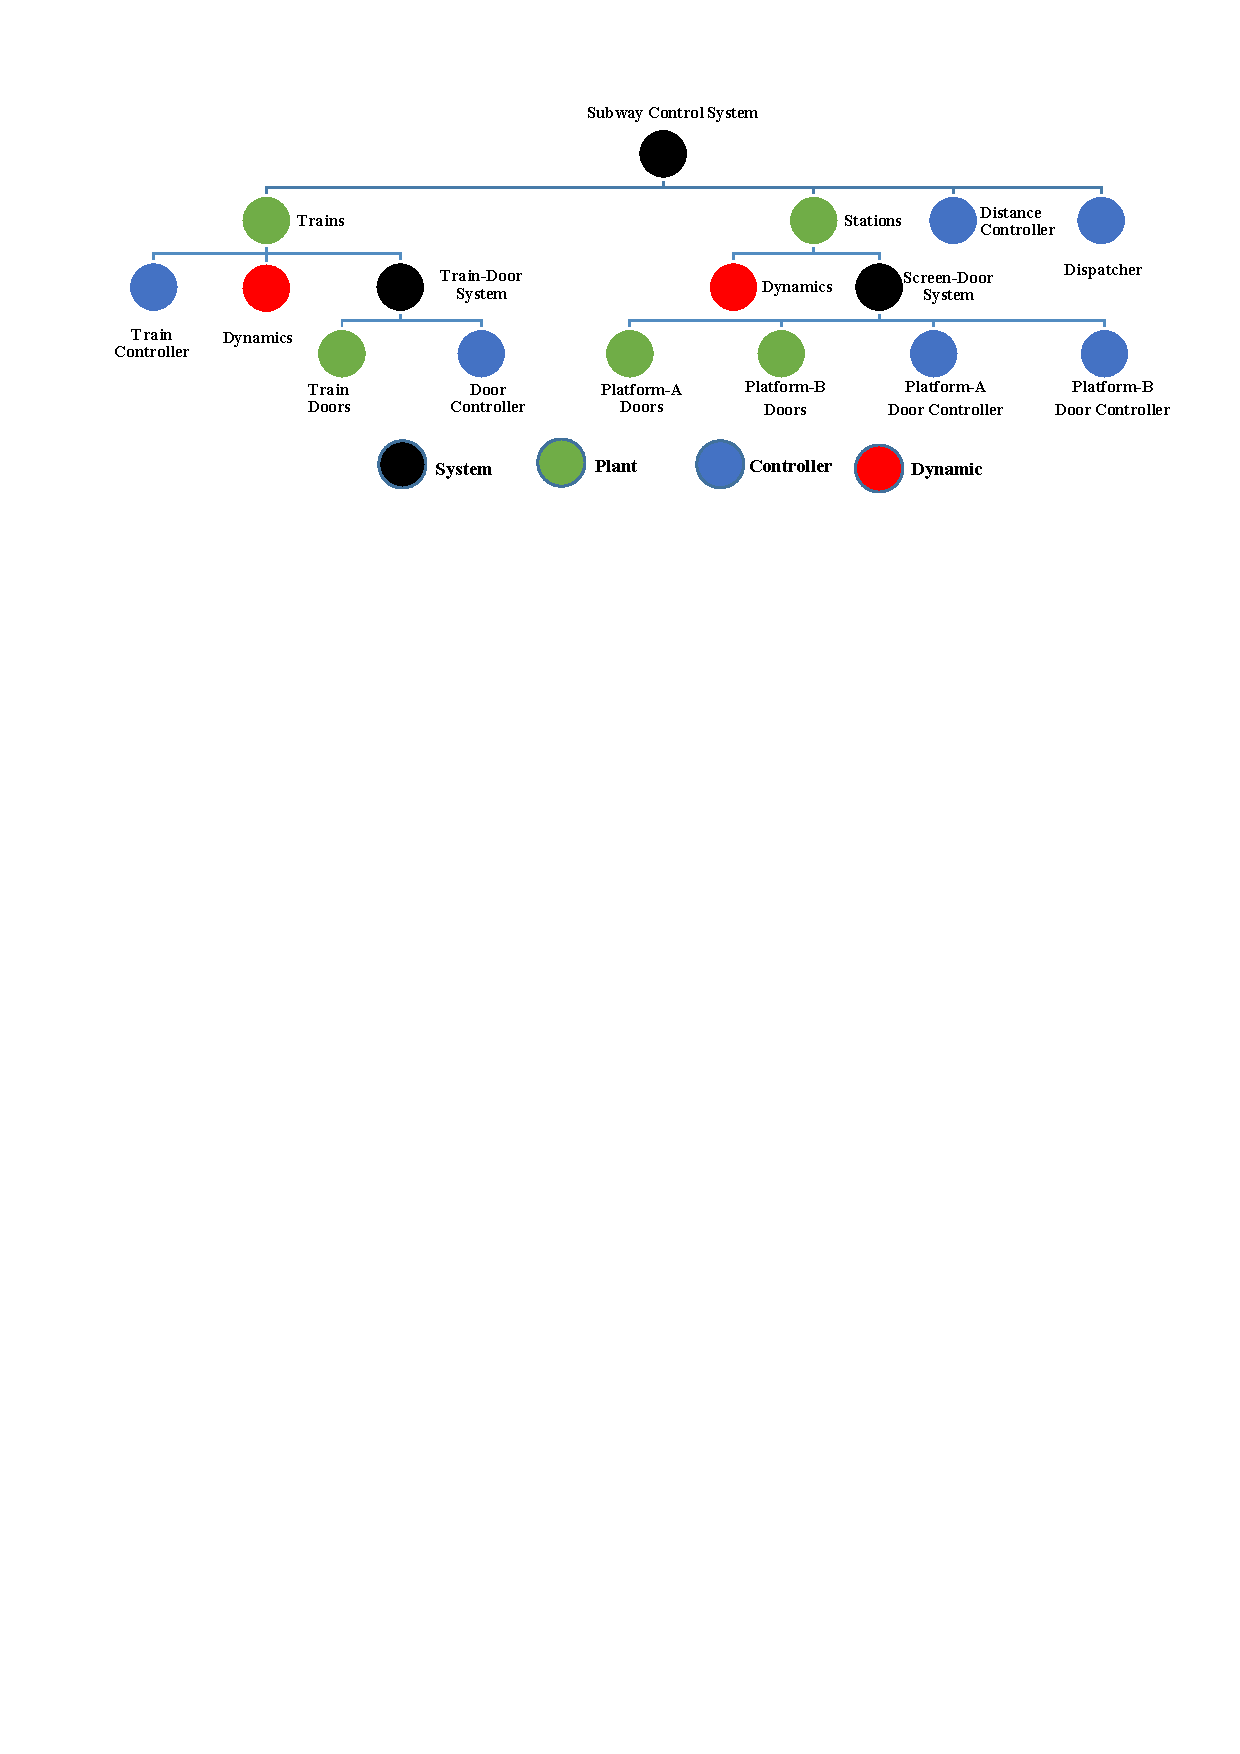
\includegraphics[width=1\linewidth]{./figs/systemstructure}
\caption[The Architecture of Subway Control System]{The Architecture of Subway Control System.
We use four key elements (i.e., System, Plant, Controller, and Dynamic) of {\apricot} to illustrate the architecture of the model.}
\label{fig:systemstructure}
\end{figure}

\begin{figure}
\centering
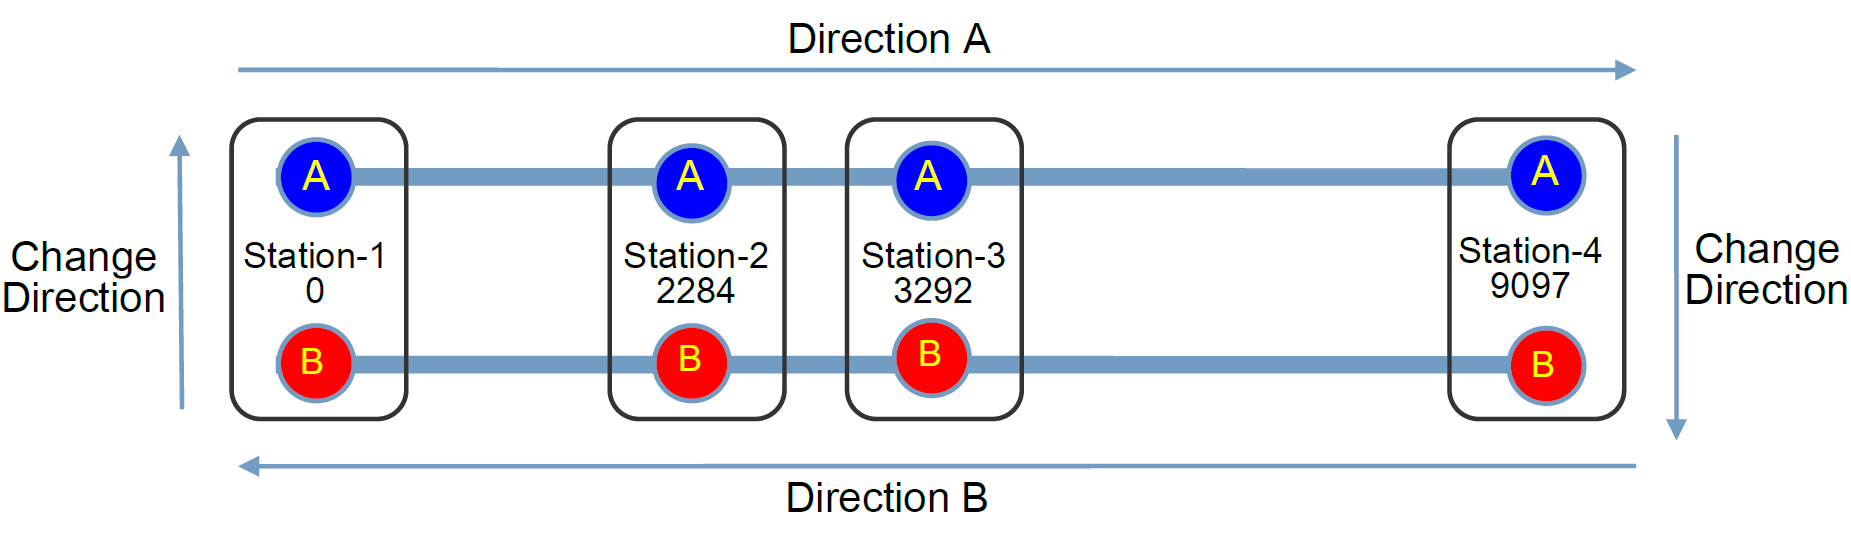
\includegraphics[width=0.8\linewidth]{./figs/sbwl}
\caption[The Topology of Subway Line]{The Topology of Subway Line. We have four stations: Station-1, 2, 3 and 4. Station-1 is a reference point, the position of the station in the subway line is 0. Station-2 is positioned at 2284, which means the distance between Station-1 and 2 is 2284 meters.}
\label{fig:sbwl}
\end{figure}



\part[Verification and Synthesis]{Formal Verification and Controller Synthesis}

\chapter{Formal Verification}

\part[Simulation and Analysis]{Simulation and Analysis}

\part[Animation and Visualization]{Animation and Visualization}

\part[Feedback-Advancement Framework]{Feedback-Advancement Framework}

\part{Conclusion}
%%%%%%%%%%%%%%%%%%%%%%%%%%%%%%%%%%%%%%%%%%%%%%%%%%%%%%
%% optional prologue or prologues
% \chapter{Chapter Title}
% \prologue{<text>}{<author attribution>}

%%%%%%%%%%%%%%%%%%%%%%%%%%%%%%%%%%%%%%%%%%%%%
% Edited Book: Author and Affiliation
%%%%%%%%%%%%%%%%%%%%%%%%%%%%%%%%%%%%%%%%%%%%%

% After \chapter{Chapter Title}, you can
% enter the author name and embed the affiliation with
% \chapterauthors{(author name, or names)
% \chapteraffil{(affiliation or affiliations)}
% }    

% For instance:
% \chapter{Chapter Title}
% \chapterauthors{G. Alvarez and R. K. Watts
% \chapteraffil{Carnegie Mellon University, Pittsburgh, Pennsylvania}

% For separate affiliations you can use \affilmark{(number)} after
% the name of a particular author and before the matching affiliation:

% For instance:
% \chapter{Chapter Title}
% \chapterauthors{George Smeal, Ph.D.\affilmark{1}, Sally Smith,
% M.D.\affilmark{2}, and Stanley Kubrick\affilmark{1}
% \chapteraffil{\affilmark{1}AT\&T Bell Laboratories
% Murray Hill, New Jersey\\
% \affilmark{2}Harvard Medical School,
% Boston, Massachusetts}
% }

%%%%%%%%%%%%%%%%%%%%%%%

%% short version of section head, or one without \\ supplied in sq. brackets.

% \section[Introduction and fugue]{Introduction\\ and fugue}
% \subsection[This is the subsection]{This is the\\ subsection}
% \subsubsection{This is the subsubsection}
% \paragraph{This is the paragraph}

% \begin{chapreferences}{widest label}
% \bibitem{<label>}Reference
% \end{chapreferences}

% optional chapter bibliography using BibTeX,
% must also have \usepackage{chapterbib} before \begin{document}
% Must use root file with \include{chap1}, \include{chap2} form.
%\bibliographystyle{plain}
%\bibliography{<your .bib file name>}

% optional appendix at the end of a chapter:
% \chapappendix{<chap appendix title>}
% \chapappendix{} % no title

%%%%%%%%%%%%%%%%%%%%%%%%%%%%%%%%%%%%%%%%%%%%%%%%%%%%%%%%%%%%%%%%
%% End Matter >>>>>>>>>>>>>>>>>>

% \appendix{<optional title for appendix at end of book>}
% \appendix{} % appendix without title

% \begin{references}{<widest label>}
% \bibitem{sampref}Here is reference.
% \end{references}

%%%%%%%%%%%%%%%%%%%%%%%%%%%%%%%%%%%%%%%%%%%%%%%%%%%%%%%%%%%%%%%%
%% Optional Problem Sets: Can use this at the end of each chapter or at end
%% of book

% \begin{problems}
% \prob
% text

% \prob
% text

% \subprob
% text

% \subprob
% text

% \prob
% text
% \end{problems}

%%%%%%%%%%%%%%%%%%%%%%%%%%%%%%%%%%%%%%%%%%%%%%%%%%%%%%%%%%%%%%%%
%% Optional Exercises: Can use this at the end of each chapter or at end
%% of book

% \begin{exercises}
% \exer
% text

% \exer
% text

% \subexer
% text

% \subexer
% text

% \exer
% text
% \end{exercises}


%%%%%%%%%%%%%%%%%%%%%%%%%%%%%%%%%%%%%%%%%%%%%%%%%%%%%%%%%%%%%%%%
%% INDEX: Use only one index command set:

%% 1) The default LaTeX Index
\printindex

%% 2) For Topic index and Author index:

% \usepackage{multind}
% \makeindex{topic}
% \makeindex{authors}
% \begin{document}
% ...
% add index terms to your book, ie,
% \index{topic}{A term to go to the topic index}
% \index{authors}{Put this author in the author index}

%% (these are Wiley commands)
%\multiprintindex{topic}{Topic index}
%\multiprintindex{authors}{Author index}

\end{document}

%%%%%%% Demo of section head containing sample macro:
%% To get a macro to expand correctly in a section head, with upper and
%% lower case math, put the definition and set the box 
%% before \begin{document}, so that when it appears in the 
%% table of contents it will also work:

\newcommand{\VT}[1]{\ensuremath{{V_{T#1}}}}

%% use a box to expand the macro before we put it into the section head:

\newbox\sectsavebox
\setbox\sectsavebox=\hbox{\boldmath\VT{xyz}}

%%%%%%%%%%%%%%%%% End Demo


Other commands, and notes on usage:

-----
Possible section head levels:
